\chapter{Installations}
\section{Installing Python}
\begin{enumerate}
\item Download Python from \url{https://www.python.org/downloads/}
\item Unzip the download file and run the installer
\item Follow the instructions on the installer
\end{enumerate}
Installation procedures for Windows and Unix based OS are similar.

\section{Installing Gurobi}
\begin{enumerate}
\item Register for an academic licenese at \url{https://http://www.gurobi.com/registration/academic-license-reg}
\item Download Gurobi Optimisation Suite at \url{http://www.gurobi.com/downloads/download-center}
\item Follow the instructions in README.txt to install the software.
\item Once the software has been installed, run 'grbgetkey' with your license as the argument (ex: grbgetkey ae36ac20-16e6-acd2-f242-4da6e765fa0a)
in your command line utility.
\end{enumerate}
Installation procedures for Windows and Unix based OS are similar.

\section{Installing or-tools}
There are a few ways to install or-tools. In this project we have chosen to install from the source. Also, installing
or-tools on Windows has slightly different steps from installing in Unix based OS.Visit
\url{https://developers.google.com/optimization/installing} for the complete instructions on installation.

\section{Installing Optaplanner}
\begin{enumerate}
\item Download Optaplanner from \url{http://www.optaplanner.org/download/download.html}
\item Unpack the download file and go to open the project folder
\item To run the optimisation suite, run runExamples.sh on Unix or runExamples.bat on Windows. Both files are located
in examples directory in the project folder
\end{enumerate}

\chapter{User Manual}
\section{Prerequisites}
\begin{enumerate}
    \item Install all the softwares in the installations section of the appendix
    \item Clone the project repository at \url{https://github.com/mombi93/or-project}
\end{enumerate}

\section{How to Run Gurobi Models}
\begin{enumerate}
    \item Edit cvrp-gurobi.py with suitable parameters
    \item run the model with python with two arguments: cvrp-gurobi.py and the path to the dataset
    (e.g python cvrp-guroby.py ../dataset/cvrp-50.txt)
    \item Once the script terminates, the optimal result will be shown.
\end{enumerate}

\section{How to Run or-tools Models}
\begin{enumerate}
    \item Go to or-tools directory.
    \item Put cvrp-or-tools.py in the /examples/python directory.
    \item Change cvrp-or-tools.py so that it takes the desired dataset and parameters.
    \item Go back to the root project directory and type make rpy EX=cvrp-or-tools
    \item Once the script terminates, the optimal result will be shown.
\end{enumerate}

\section{How to Run Optaplanner Models}
\subsection{Running Parsed Models}
\begin{enumerate}
    \item copy the 'solved' and 'unsolved' folder in this repository to the directory where the XML inputs for vehicle
    routing problems are kept. They are kept in the following path : /examples/sources/data/vehiclerouting of
    the Optaplanner optimisation suite.
    \item run Optaplanner using ./runExamples.sh on Unix or ./runExamples.bat on windows from its root directory.
    \item Using the GUI, select the desired model and press the solve button on the top right hand corner of the optimisation suite.
\end{enumerate}

\subsection{Parsing Models}
We use xml-gen.py to parse the given datasets into XML files. The script only process datasets that have certain schema.
\begin{enumerate}
    \item Edit xml-gen.py in this project's repository (under the optaplanner directory) to locate the right dataset files
    and parameters.
    \item Run the script using python to obtain the desired XML file.
\end{enumerate}

\subsection{Retrieving the Optimal Routes}
\begin{enumerate}
    \item Edit rt-dist-calc.py in this project's repository (under the optaplanner directory)to locate the solved Optaplanner model and
    the file where the file should be written.
    \item Run the script using python to write the optimal routes to the specified file.
\end{enumerate}

\subsection{Computing Total distance in kilometers}
\begin{enumerate}
    \item Edit rt-dist-calc.py in this project's repository (under the optaplanner directory) to calculate the total distance
    \item Run the script using python to get the distance in kilometers.
\end{enumerate}


\chapter{Datasets}
\section{Node Number to Postal Code Dictionary}
\vspace{0.5cm}
\lstinputlisting[language=Python]{./dataset/nodes-dict.txt}

\section{Dataset Description Table}
\begin{table}[!ht]
    \begin{center}
        \begin{tabular}{ | l| l |l| l |l|p{5cm}|}
        \hline
        Type & Name & Customers &  Vehicles & Capacity & Description \\ \hline
        Test & T-VRP-9 & 9 & 3 & 4 & This is benchmark dataset that is used if the LP models are implemented correctly. The model of this dataset
        has a known best solution\\ \hline
        Test & T-VRP-60 & 60 & 5 & 15 & This dataset uses the first 60 node of the P-VRP-227 dataset. It is used for to model a CVRP instance that is
        similar to the given problem.
        performance of the chosen LP tools on.\\\hline
        Benchmark & A-n32-k5 & 32 & 5 & 100 & This is the benchmark dataset for a CVRP model that is used to analyse the performance the chosen LP tools.\\\hline
        Benchmark & A-n44-k6 & 44 & 6 & 100 & This is the benchmark dataset for a CVRP model that is used to analyse the performance the chosen LP tools.\\\hline
        Benchmark & A-n53-k7 & 53 & 7 & 100 & This is the benchmark dataset for a CVRP model that is used to analyse the performance the chosen LP tools.\\\hline
        Benchmark & A-n65-k9 & 65 & 9 & 100 & This is the benchmark dataset for a CVRP model that is used to analyse the performance the chosen LP tools.\\\hline
        Benchmark & A-n80-k10 & 80 & 10 & 100 & This is the benchmark dataset for a CVRP model that is used to analyse the performance the chosen LP tools.\\\hline
        Problem & P-VRP-227 & 227 & 8 & 29 & This dataset is the problem dataset from Furnish. It is used to model both CVRP and CVRPTW models
        in this project.\\\hline
        \end{tabular}
        \caption{Datasets description}
        \label{table:dataset_description}
    \end{center}
\end{table}

\chapter{Evaluation Data and Results}

\section{Vehicle Routes}
\begin{table}[!ht]
\centering
\begin{tabular}{|l|l|}
\hline
Vehicle No         & Order of visit                                                                         \\ \hline
\multirow{2}{*}{1} & \multirow{2}{*}{\begin{tabular}[c]{@{}l@{}}48, 57, 75, 70, 102, 87, 79, 96, 97, 91, 144, 126, 146, 145,\\ 163, 188, 182, 187, 171, 189, 143, 62, 156, 167, 134, 76, 45, 29\end{tabular}} \\
                   &                                                                                  \\ \hline
\multirow{2}{*}{2} & \multirow{2}{*}{\begin{tabular}[c]{@{}l@{}}24, 54, 68, 67, 85, 80, 110, 152, 180, 191, 193, 196, 181, 147,\\ 175, 113, 108, 83, 78, 130, 136, 154, 105, 73, 53, 23, 44, 41, 22\end{tabular}}  \\
                   &                                                                                  \\ \hline
\multirow{2}{*}{3} & \multirow{2}{*}{\begin{tabular}[c]{@{}l@{}}25, 40, 127, 107, 141, 199, 202, 209, 192, 213, 217, 222, 201,\\ 210, 208, 204, 206, 214, 207, 195, 205, 112, 92, 88, 104, 93\end{tabular}} \\
                   &                                                                                  \\ \hline
\multirow{2}{*}{4} & \multirow{2}{*}{\begin{tabular}[c]{@{}l@{}}32, 47, 59, 21, 26, 43, 31, 114, 98, 178, 172, 176, 161, 165,\\ 185, 216, 225, 218, 226, 227, 224, 220, 223, 215, 184, 103, 74, 63, 37\end{tabular}}  \\
                   &                                                                                  \\ \hline
\multirow{2}{*}{5} & \multirow{2}{*}{\begin{tabular}[c]{@{}l@{}}36, 60, 56, 128, 153, 140, 133, 166, 139, 162, 194, 183, 168,\\ 173, 155, 135, 115, 95, 72, 77, 94, 61, 99, 124, 86, 109, 123\end{tabular}}  \\
                   &                                                                                  \\ \hline
\multirow{2}{*}{6} & \multirow{2}{*}{\begin{tabular}[c]{@{}l@{}}71, 33, 69, 46, 42, 82, 65, 131, 132, 164, 169, 150, 177, 190,\\ 125, 116, 66, 118, 119, 106, 101, 138, 84, 90, 120, 142, 121, 111, 52\end{tabular}}  \\
                   &                                                                                  \\ \hline
\multirow{2}{*}{7} & \multirow{2}{*}{\begin{tabular}[c]{@{}l@{}}17, 20, 30, 19, 15, 13, 14, 35, 34, 38, 39, 28, 64, 58, 49, 51,\\ 55, 16, 18, 12, 50, 9, 10, 11, 7, 8, 2, 4, 5\end{tabular}}  \\
                   &                                                                                  \\ \hline
\multirow{2}{*}{8} & \multirow{2}{*}{\begin{tabular}[c]{@{}l@{}}3, 6, 89, 151, 129, 157, 122, 137, 159, 158, 117, 174, 198, 186,\\ 212, 211, 221, 219, 200, 203, 197, 179, 170, 149, 160, 148, 100, 81, 27\end{tabular}}  \\
                   &                                                                                  \\ \hline
\end{tabular}
\caption{Routes for CVRP Model}
\label{cvrp-routes}
\end{table}

\begin{table}[ht!]
\centering
\begin{tabular}{|l|l|}
\hline
Vehicle No         & Order of visit                                                                           \\ \hline
\multirow{2}{*}{1} & \multirow{2}{*}{\begin{tabular}[c]{@{}l@{}}3, 151, 157, 85, 129, 122, 137, 159, 117, 158, 174, 136, 108, 95,\\ 113, 198, 179, 197, 203, 212, 211, 221, 219, 200, 89, 8, 7, 2\end{tabular}} \\
                   &                                                                                  \\ \hline
\multirow{2}{*}{2} & \multirow{2}{*}{\begin{tabular}[c]{@{}l@{}}24, 40, 41, 27, 81, 148, 110, 78, 72, 83, 80, 77, 115, 149, 186,\\ 191, 181, 196, 193, 152, 133, 61, 140, 94, 124, 99, 54, 44\end{tabular}}  \\
                   &                                                                                  \\ \hline
\multirow{2}{*}{3} & \multirow{2}{*}{\begin{tabular}[c]{@{}l@{}}25, 60, 56, 86, 100, 135, 166, 139, 155, 194, 162, 183, 173, 168,\\ 170, 160, 180, 175, 147, 130, 154, 105, 73, 68, 67, 53, 23, 36, 22\end{tabular}} \\
                   &                                                                                  \\ \hline
\multirow{2}{*}{4} & \multirow{2}{*}{\begin{tabular}[c]{@{}l@{}}55, 37, 63, 31, 93, 123, 109, 127, 141, 128, 153, 107, 199, 202,\\ 209, 192, 201, 210, 222, 217, 213, 204, 208, 205, 185, 172, 91, 104, 48\end{tabular}}  \\
                   &                                                                                  \\ \hline
\multirow{2}{*}{5} & \multirow{2}{*}{\begin{tabular}[c]{@{}l@{}}75, 102, 103, 145, 176, 184, 215, 220, 223, 224, 227, 226, 225,\\ 216, 218, 195, 214, 207, 206, 178, 161, 165, 112, 98, 92, 88, 114, 43, 26\end{tabular}}  \\
                   &                                                                                  \\ \hline
\multirow{2}{*}{6} & \multirow{2}{*}{\begin{tabular}[c]{@{}l@{}}52, 111, 118, 119, 106, 101, 142, 121, 120, 90, 84, 190, 177,\\ 116, 125, 164, 169, 150, 134, 132, 131, 82, 65, 76, 46, 69, 70, 57\end{tabular}}  \\
                   &                                                                                  \\ \hline
\multirow{2}{*}{7} & \multirow{2}{*}{\begin{tabular}[c]{@{}l@{}}32, 47, 59, 21, 87, 97, 126, 163, 146, 144, 188, 182, 187, 96,\\ 79, 74, 143, 62, 156, 189, 171, 167, 45, 42, 29, 33, 71\end{tabular}}  \\
                   &                                                                                  \\ \hline
\multirow{2}{*}{8} & \multirow{2}{*}{\begin{tabular}[c]{@{}l@{}}19, 20, 30, 17, 14, 13, 15, 35, 34, 38, 28, 39, 64, 138, 66, 58,\\ 49, 51, 4, 5, 6, 11, 16, 10, 9, 50, 12, 18\end{tabular}}  \\
                   &                                                                                  \\ \hline
\end{tabular}
\caption{Routes for CVRPTW Model}
\label{cvrptw-routes}
\end{table}
\vspace{5cm}
\section{Route Visualisation}

\begin{figure}[ht!]
  \centering
    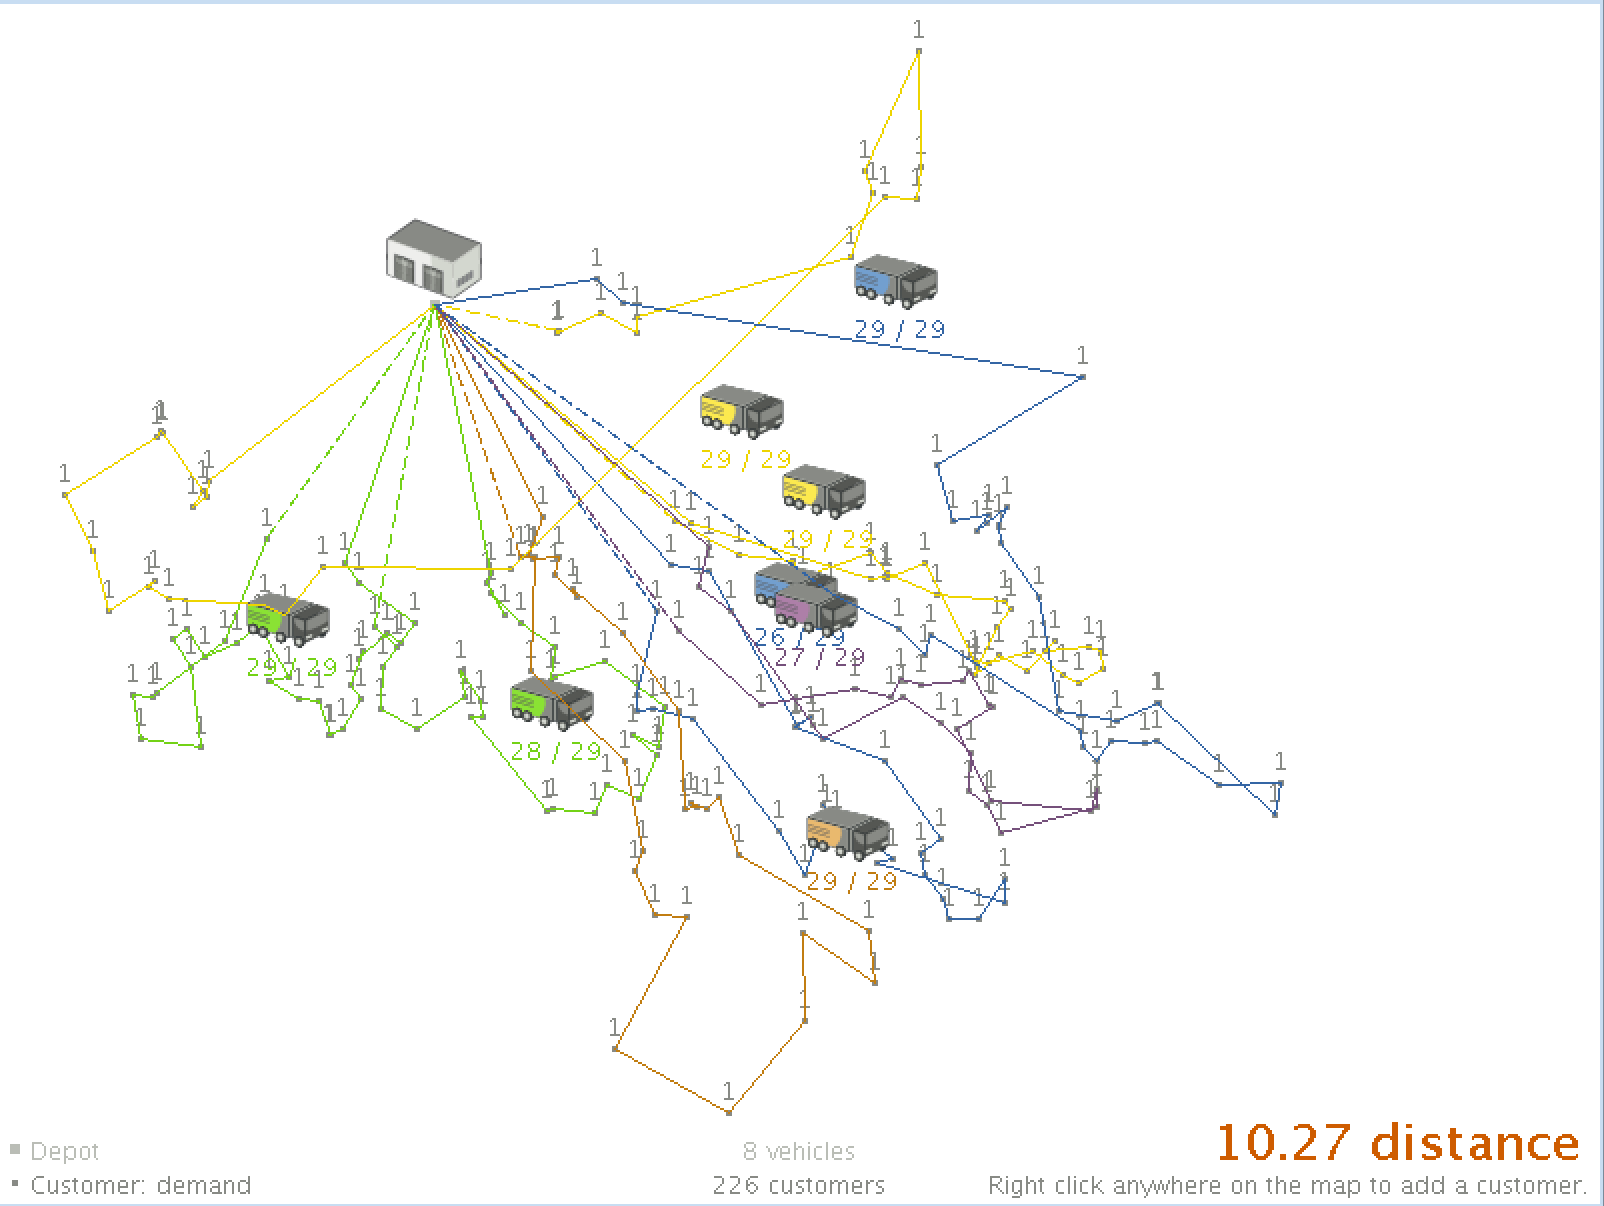
\includegraphics[width=0.85\textwidth]{227-cvrp.png}
    \caption{Visualisation of CVRP Model}
\end{figure}
\begin{figure}[!ht]
  \centering
    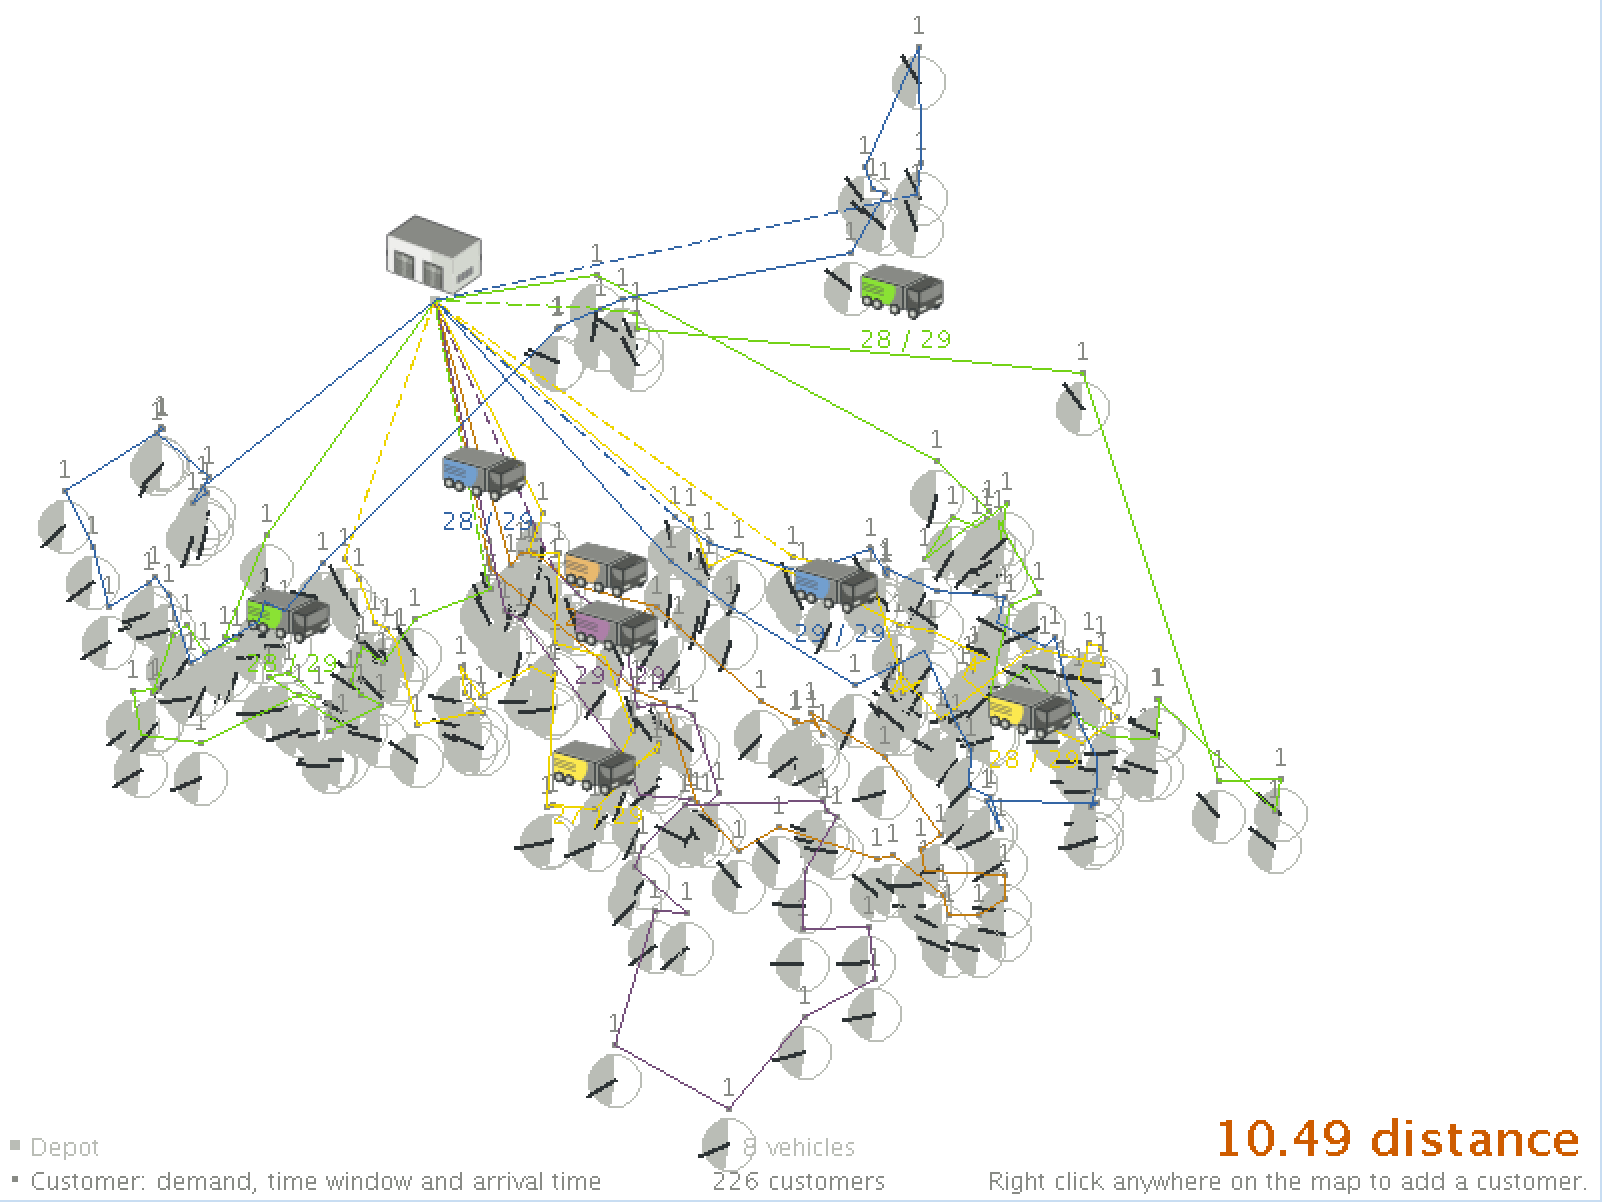
\includegraphics[width=0.85\textwidth]{227-cvrptw.png}
    \caption{Visualisation of CVRPTW Model}
\end{figure}

\chapter{Project Plan and Interim Report}
\section{Project Plan}
\textbf{Final Year Project Plan}

\textbf{Name}: Muhammad Rafdi

\textbf{Project Title}: Using Integer Linear Programming to Solve Routing Problems (Tentative)

\textbf{Supervisor Name}: Daniel Hulme

\textbf{Aims}: The aim of this project is to model routing problem based on actual data sets in the real world and obtain their optimal solution(s) through integer linear programming formulations.

\textbf{Objectives}:
\begin{enumerate}
    \item Preliminary: Explore Linear and Integer programming to model problems in terms of linear programs and find their optimal solutions.
    \item Preliminary: Model routing problems in terms of Travelling salesman problem (or one of its variants), which would then be solved using Integer Programming formulations.
    \item Use the actual routing data set for the TSP model and solve it using integer programming. This may be done in two steps. The first step assume little or negligible constraint on the data set (weather, roadblock etc). Once that has been solved, proceed to second step in which all the constraints in the real world would be included.
    \item Use variety of integer programming formulations and formats and analyse their results.
    \item Additional would-like-to-have requirements such as visualisation, creating a web platform etc.
\end{enumerate}

\textbf{Expected outcomes/deliverables}:
\begin{enumerate}
    \item Successfully model the routing problem into a suitable model for Integer programming.
    \item Obtain the optimal solution(s) to the routing problem given the data set with both minimal and actual real life constraints.
    \item Compare and contrast the results using different integer programming formulations.
    \item Fulfil any additional objectives that may be added.
\end{enumerate}

\textbf{Work plan}:
\begin{enumerate}
    \item Early October 2015 - Mid December 2015: Research on linear and integer programming and literature review. Also learn to use linear programming solver such as GLPK or Matlab.
    \item Mid December 2015 - Early January 2016:
    \begin{enumerate}
        \item Learn how to model simple routing problems in terms of TSP
        \item Analyse routing data sets to identify its objectives and constraints.
        \item Start writing the report for the project.
    \end{enumerate}
     \item Early January 2016 - mid March 2016:
     \begin{enumerate}
        \item Obtain optimal solutions from the problem (which have been modelled from data set) using different formulations and formats.
        \item Tabulate their results appropriately and compare and contrast their results.
        \item Start working on additional requirements.
    \end{enumerate}
    \item Mid March 2016 - End of April:
    \begin {enumerate}
        \item Finalise the project report.
        \item Finish up any additional requirements.
    \end{enumerate}
\end{enumerate}

\section{Interim Report}

\textbf{Final Year Project Interim Report}

\textbf{Name}: Muhammad Rafdi

\textbf{Project Title}: Using Integer Programming to Solve Routing Problems.

\textbf{Current Project Title}: Integer Programming to Solve Routing Optimisation
Problem

\textbf{Supervisor}: Daniel Hulme

\textbf{Progress Made}: I spent majority of the term learning integer programming and looking at different problems to optimise.
I took an interest in optimising routing problems such as the travelling salesman problem. After speaking to my supervisor,
 he advised me to work on a specific a data set, which is based on a real life situation.

Since then, I have been working towards optimising the problem given the dataset. Firstly, I looked at literatures on
how to model the problem correctly, such as adding subtour elimination constraints. Secondly, I have installed all the
required software, such as GLPK and Gurobi Optimisation suite. I have also set up a Git repository that contains the
simple mathematical model that solves a simpler instance the problem and the travel matrix of the data that has been
cleaned to fit to the given model.

\textbf{Remaining Work}: In order to finish the project, I need to be able to correctly optimise the problem based on the given
dataset. This means creating a model that accurately represents the problem and cleaning up the dataset so that it fits
with the model. A comparison should also be made to compare the different results that are generated from different
variation of models and software. Finally, it would be a bonus point if a recommendation could be made based on
results obtained.

\textbf{Supervisor Signature}:  Approved as per the email.


\chapter{Code Listings}

\section{cvrp-gurobi.py - CVRP Model Implementation in Gurobi}
\lstinputlisting[language=Python]{./python/cvrp-gurobi.py}

\section{cvrp-or-tools.py - CVRP Model Implementation in or-tools}
\lstinputlisting[language=Python]{./python/cvrp-or-tools.py}

\section{xml-gen.py - XML Generator Script for Optaplanner}
\lstinputlisting[language=Python]{./optaplanner/xml-gen.py}

\section{rt-dist-calc.py - Distance Utility Script}
\lstinputlisting[language=Python]{./optaplanner/rt-dist-calc.py}
